\documentclass[14pt,a4paper]{article}
\usepackage[utf8]{inputenc}
\usepackage[russianb]{babel}
\usepackage[left=1.5cm,right=1.5cm,top=2cm,bottom=2.5cm]{geometry}
\usepackage{setspace}
\usepackage{indentfirst}
\usepackage{amssymb}
\usepackage{amsmath}
\usepackage{bm}

\usepackage{array}
\usepackage[pdftex]{graphicx}
\usepackage{comment}
\usepackage[table,xcdraw]{xcolor}


\usepackage{verbatim}


\graphicspath{{images/}}
\renewcommand{\baselinestretch}{1.3}

\begin{document}

Для визуализации алгоритма Черепахи напишем программу, используя библиотеку Turtle. Программа должна нарисовать фигуру, заданную алгоритмом, а также точки с целочисленными координатами, чтобы можно было посчитать, сколько точек внутри области, ограниченной фигурой. Для управления масштабом картинки будем использовать переменную scale: все координаты и перемещения умножаются на неё.

\begin{verbatim}
from turtle import *

# Ускорение отрисовки
tracer(0)
# Поворот влево, чтобы Черепаха смотрел вдоль оси ординат
left(90)

# Масштаб
scale = 40

# Повтори 7
for _ in range(7):
    # Вперёд 10
    forward(10 * scale)
    # Направо 10
    right(120)


# Поднимаем хвост, чтобы нарисовать точки
up()
# Рисуем точки с координатами от -20 до 20
for x in range(-20, 20):
    for y in range(-20, 20):
        # Перемещаем Черепаху в точку (x, y)
        goto(x * scale, y * scale)
        # Зелёная точка
        dot(5, "green")


# Отрисовать рисунок
update()
# Конец программы, чтобы рисунок сразу не закрылся
done()
\end{verbatim}

Получим следующий рисунок:
\begin{center}
    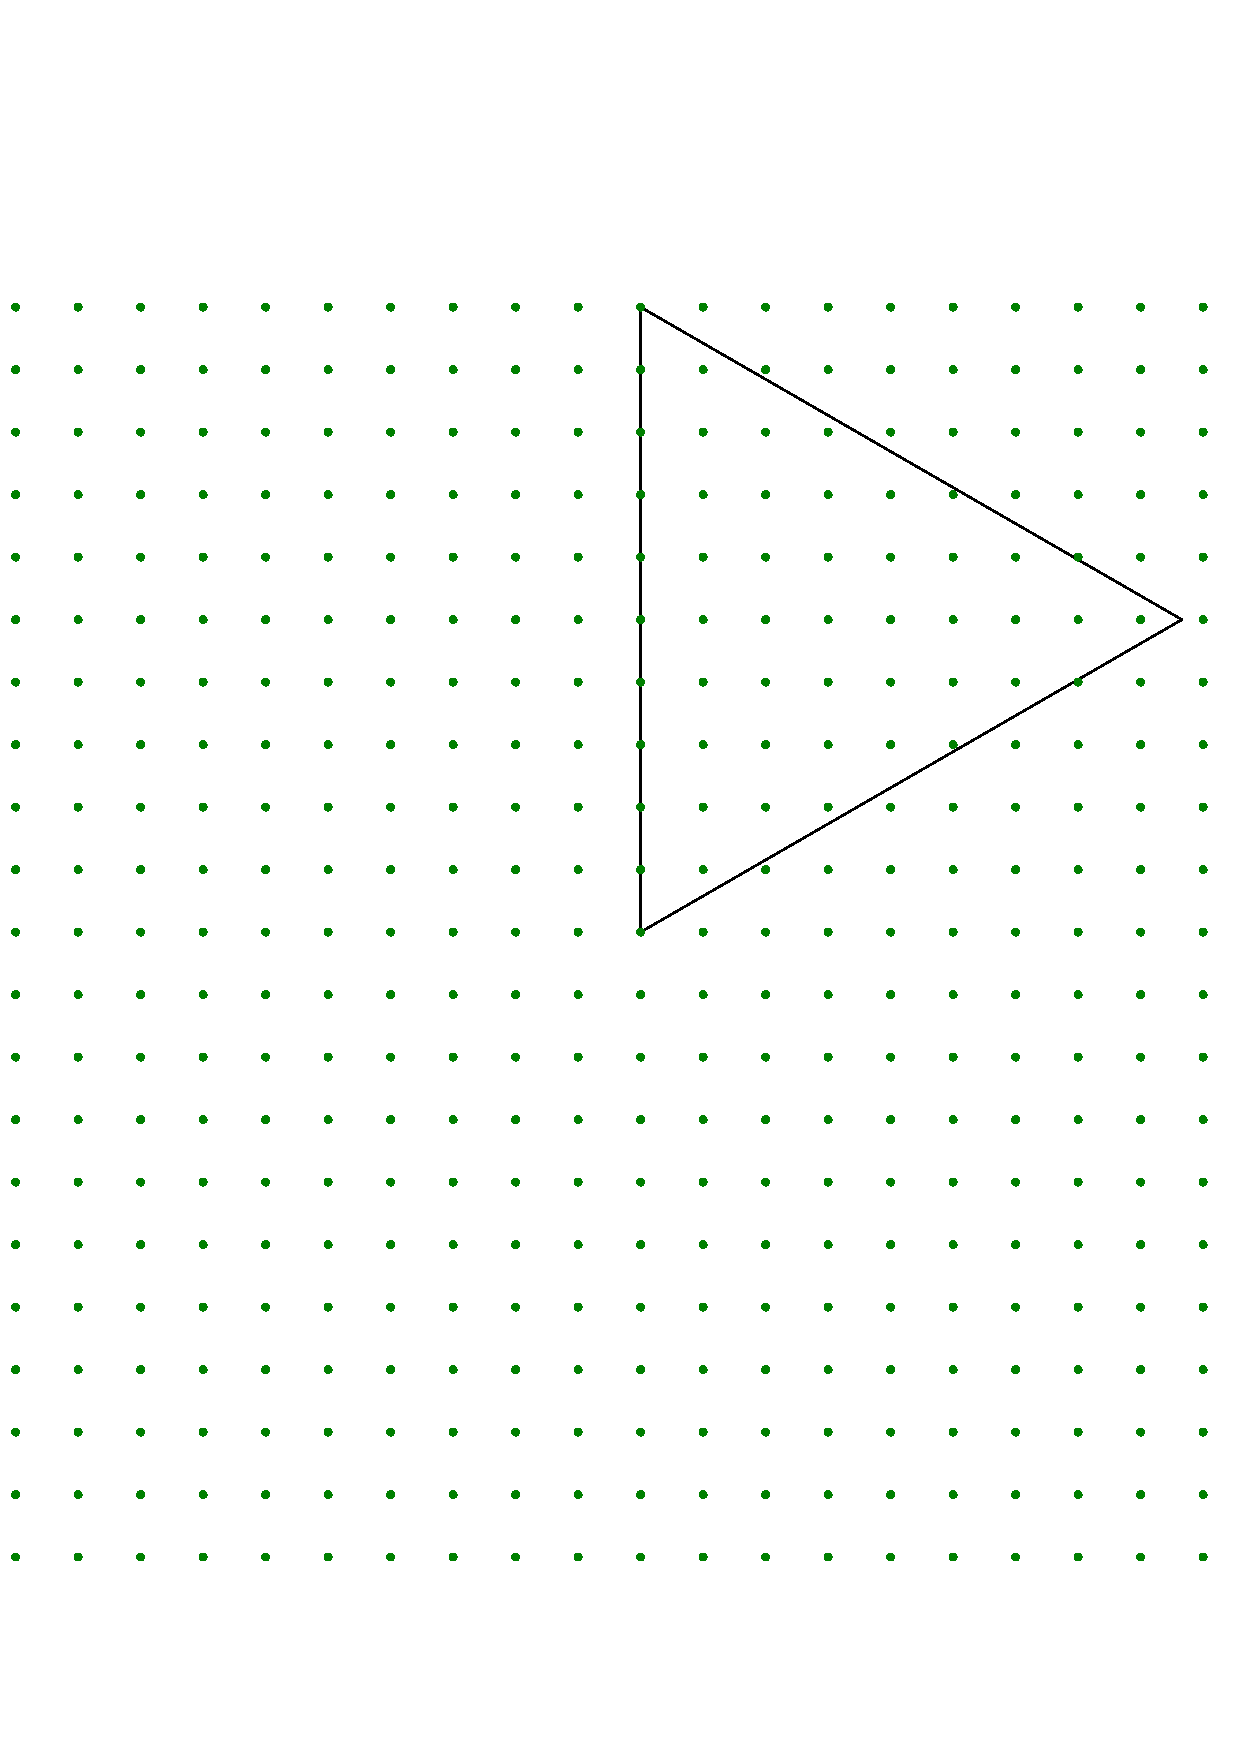
\includegraphics[width=0.4\textwidth]{figure.png}
\end{center}

Посчитаем точки внутри и получим ответ -- 38.

\end{document}
